% +------------------------------------------------------------------------+
% | CGAL Reference Manual:  partition_2.tex
% +------------------------------------------------------------------------+
% | Planar polygon partitioning
% |
% | 28.07.2000   Susan Hert
% |
% +------------------------------------------------------------------------+


% =============================================================================
% The CGAL Developers' Manual
% -----------------------------------------------------------------------------
% file   : index_see.tex
% authors: Susan Hert <hert@mpi-sb.mpg.de>
% -----------------------------------------------------------------------------
% $Revision$
% $Date$
% =============================================================================

\ccIndexSubsubitemSeeAlso{traits class}{kernel as a}{kernel traits}

\index{documentation!specification|see{manuals}}
\index{PostScript manual|see{manuals, PostScript}}
\index{HTML manual|see{manuals, HTML}}
\index{manuals!reference|see{reference manual}}
\index{manuals!users'|see{users' manual}}
\index{section headings!manual|see{manual, section headings}}
\index{manuals!tools|see{tools, manual}}
\index{cgal_namespace@\cgal\ namespace|see{namespaces, \cgal}}

\index{files|see{source files}}

\index{output iterators|see{iterators, output}}
\index{input iterators|see{iterators, input}}

\index{geometry kernel|see{kernels}}

\index{demo\ programs!on the web|see{Java demo server}}
\index{demo\ programs!Java|see{Java demo server}}
\index{Cartesian!kernel|see{kernels, \ccc{Cartesian}}}
\index{homogeneous!kernel|see{kernels, \ccc{homogeneous}}}

\index{flag!workaround|see{workaround flags}}
\index{flag!configuration|see{workaround flags}}
\index{memory allocator|see{allocator}}


\section{Introduction}
\label{sec:partition_2_intro}
A {\em partition}\ccIndexMainItemDef{partition} of a polygon $P$ is a set of 
polygons % $P_1, \ldots, P_p$ 
such that the 
interiors of the polygons do not intersect and the union of the polygons 
is equal to the interior of the original polygon $P$.  
This chapter describes functions for partitioning
planar polygons into two types of subpolygons --- $y$-monotone polygons and
convex polygons.  The partitions are produced without introducing new
(Steiner) vertices. 

All the partitioning functions present the same interface to
the user.  That is, the user provides a pair of input iterators, \ccc{first}
and \ccc{beyond}, an output iterator \ccc{result},  and a traits class 
\ccc{traits}. The points in the range [\ccc{first}, \ccc{beyond}) are assumed
to define a simple polygon whose vertices are in counterclockwise order.
The computed partition polygons, whose vertices are also oriented 
counterclockwise, are written to the sequence starting at position
\ccc{result} and the past-the-end interator for the resulting sequence of
polygons is returned.  The traits classes for the functions specify the types
of the input points and output polygons as well as a few other types and
function objects that are required by the various algorithms.


\section{Monotone Partitioning}
\label{sec:partition_2_monotone}
\ccIndexSubitem{polygon partitioning}{y-monotone}
A {\em $y$-monotone polygon}\ccIndexMainItemDef{y-monotone polygon}
is a polygon whose vertices $v_1, \ldots, v_n$ can be divided into two chains 
$v_1, \ldots, v_k$ and $v_k, \ldots, v_n, v_1$, such that any horizontal line 
intersects either chain at most once.  For producing a $y$-monotone partition 
of a given polygon, the sweep-line algorithm 
presented in \cite{bkos-cgaa-97} is implemented by the function
\ccc{y_monotone_partition_2}\ccIndexGlobalFunction{y_monotone_partition_2}.  
This algorithm runs in $O(n \log n)$ time and requires $O(n)$ space.
This algorithm does not guarantee a bound on the number of polygons 
produced with respect to the opitmal number.

For checking the validity of the partitions produced by 
\ccc{y_monotone_partition_2}, we provide a function \ccc{is_y_monotone_2}, 
which determines if a sequence of points in 2D defines a $y$-monotone
polygon or not.


\begin{figure}
\begin{ccHtmlOnly}
<CENTER>
<TABLE CELLSPACING=40>
</TR>
<TD>
<IMG BORDER=0 SRC=Trier.opt_cvx.gif ALIGN=CENTER ALT="Optimal Convex Partition o
f Trier">
</TD>
<TD>
<IMG BORDER=0 SRC=Idar-Oberstein.appx_cvx.gif ALIGN=CENTER ALT="Approx. Optimal
Convex Partition of Idar-Oberstein">
</TD>
</TR>
</TABLE>
</CENTER>
\end{ccHtmlOnly}

\begin{ccTexOnly}
\begin{center}
\includegraphics[width=6.5cm]{Trier.opt_cvx.ps}
\includegraphics[width=6.5cm]{Idar-Oberstein.appx_cvx.ps}
%\leavevmode\epsfxsize8cm\epsffile{saarhull.eps}
\end{center}
\end{ccTexOnly}
\caption{Examples of an optimal convex partition (left) and an approximately
optimal convex partition (right).}
\end{figure}


\section{Convex Partitioning}
\label{sec:partition_2_convex}
%A {\em convex polygon}%
%\ccIndexMainItemDef{convex polygon} is a polygon for which any segment
%connecting two points on the boundary of the polygon lies completely in
%the interior of the polygon.
%
\ccIndexSubitemBegin{polygon partitioning}{convex}
Three functions are provided for producing convex partitions of polygons.
One produces a partition that is optimal in the number of pieces. 
The other two functions produce approximately optimal convex partitions.
Both these functions produce convex decompositions by first decomposing the 
polygon into simpler polygons; the first uses a triangulation and the second a
monotone partition.  These two functions both guarantee that they will produce 
no more than four times the optimal number of convex pieces but they differ in 
their runtime complexities.  Though the triangulation-based approximation
algorithm often results in fewer convex pieces, this is not always the case.

An optimal convex partition can be produced using the function
\ccc{optimal_convex_partition_2}.%
\ccIndexGlobalFunction{optimal_convex_partition_2} 
\ccIndexSubsubitem{polygon partitioning}{convex}{optimal}
This function provides an
implementation of Greene's dynamic programming algorithm for optimal
partitioning \cite{g-dpcp-83}. 
This algorithm requires $O(n^4)$ time and $O(n^3)$ space in the worst case.  
%As a preprocessing step, this algorithm requires that a vertex visibility
%graph of the polygon be built.  This is done using the algorithm of
%Overmars and Welzl \cite{ow-nmcvg-88} for computing the visibility graph
%of a set of nonintersecting line segments in the plane, adapted to handle
%points that are not in general position and for the particular case that the
%segments form a polygon (and thus segments that lie completely outside the
%polygon are considered to be invisible).  This algorithm $O(n^2)$ time and 
%$O(n)$ space to compute a visibility graph for $n$ segments.

The function
\ccIndexSubsubitem{polygon partitioning}{convex}{approximately optimal}
\ccc{approx_convex_partition_2}\ccIndexGlobalFunction{approx_convex_partition_2}
implements the simple approximation algorithm of Hertel and Mehlhorn 
\cite{hm-ftsp-83} that 
produces a convex partitioning of a polygon from a triangulation by 
throwing out unnecessary triangulation edges.
The triangulation used in this function is one produced by the
2-dimensional constrained triangulation
package of \cgal.  For a given triangulation, this convex partitioning 
algorithm requires $O(n)$ time and space to construct a decomposition into 
no more than four times the optimal number of convex pieces.

\ccIndexSubsubitem{polygon partitioning}{convex}{approximately optimal}
The sweep-line approximation algorithm of Greene \cite{g-dpcp-83}, which, 
given a monotone partition of a polygon, produces a convex partition in 
$O(n \log n)$ time and $O(n)$ space, is implemented
by the function \ccc{greene_approx_convex_partition_2}%
\ccIndexGlobalFunction{greene_approx_convex_partition_2}.  The function
\ccc{y_monotone_partition} described in Section~\ref{partition_2_monotone}
is used to produce the monotone
partition.  This algorithm provides the same worst-case approximation guarantee 
as the algorithm of Hertel and Mehlhorn implemented with
\ccc{approx_convex_partition_2} but can sometimes produce better
results ({\em i.e.}, convex partitions with fewer pieces).
\ccIndexSubitemEnd{polygon partitioning}{convex}


